\startchapter{Simplified Molecular Model} \label{ch:3}

\section{Description}
The goal of Chapter \ref{ch:3} is to introduce the formulas used to describe our LP model. As well as exploring the properties of our LP model by using a toy molecule. This toy molecule contains limited vibration modesf. By doing so, the nature of the LP model we use to study the spectral information can be carefully analyzed. Our goal is to figure out with the the spectral information available, could LP model we use output any valuable information. \\

The toy molecule contains $4$ vibration modes. Theses vibrational peaks are at frequencies of $2850, 2960, 3050$ and $3200$. The widths of the peaks are $5, 10, 5$ and $15~cm^{-1}$, respectively. The amplitudes of the peak are $1, 0.7, -0.2$ and $0.5~cm^{-1}$, respectively. The comparing angles of the peaks are $15, 90, 0$ and $60$. (TODO: check with Dennis, how to further explain those comparing angles?)  \\

For the toy model, only IR spectroscopy is considered. Because we want to limit the complication that comes from the parameters needed to describe the real molecules. Equation \ref{eq:3.1} is used to generate the $cosine$-polarized IR spectrum. Both $\phi$ and $\psi$ Euler angles are integrated, only the difference on angle $\theta$ is considered. \\

\begin{eqnarray} \label{eq:3.1}
& f_{\theta}(x) = \displaystyle\sum^{4}_{q=1} A_q^2 * cos^2(\theta - \theta_q)\frac{\gamma^2}{(x- \omega_{\rm q})^2 + \gamma^2} 
\end{eqnarray}
where $A$ is the amplitude, $\theta_{q}$ is the comparing angle, $\gamma$ is the width, and $\omega_{\rm q}$ is the frequency. (TODO: Double check the correct meaning of each symbol) Ten candidates are produced with $10$ different $\theta$ values as follows: $0^{\circ}$, $10^{\circ}$, $20^{\circ}$, $30^{\circ}$, $40^{\circ}$, $50^{\circ}$, $60^{\circ}$, $70^{\circ}$, $80^{\circ}$, $90^{\circ}$. Their spectra are shown in Figure \ref{fig:3.1}. The 10 candidates have peaks at the same frequencies. The spectral signal for candidates is comparatively strong at each peak. \\

\begin{figure}[!ht] 
\centering
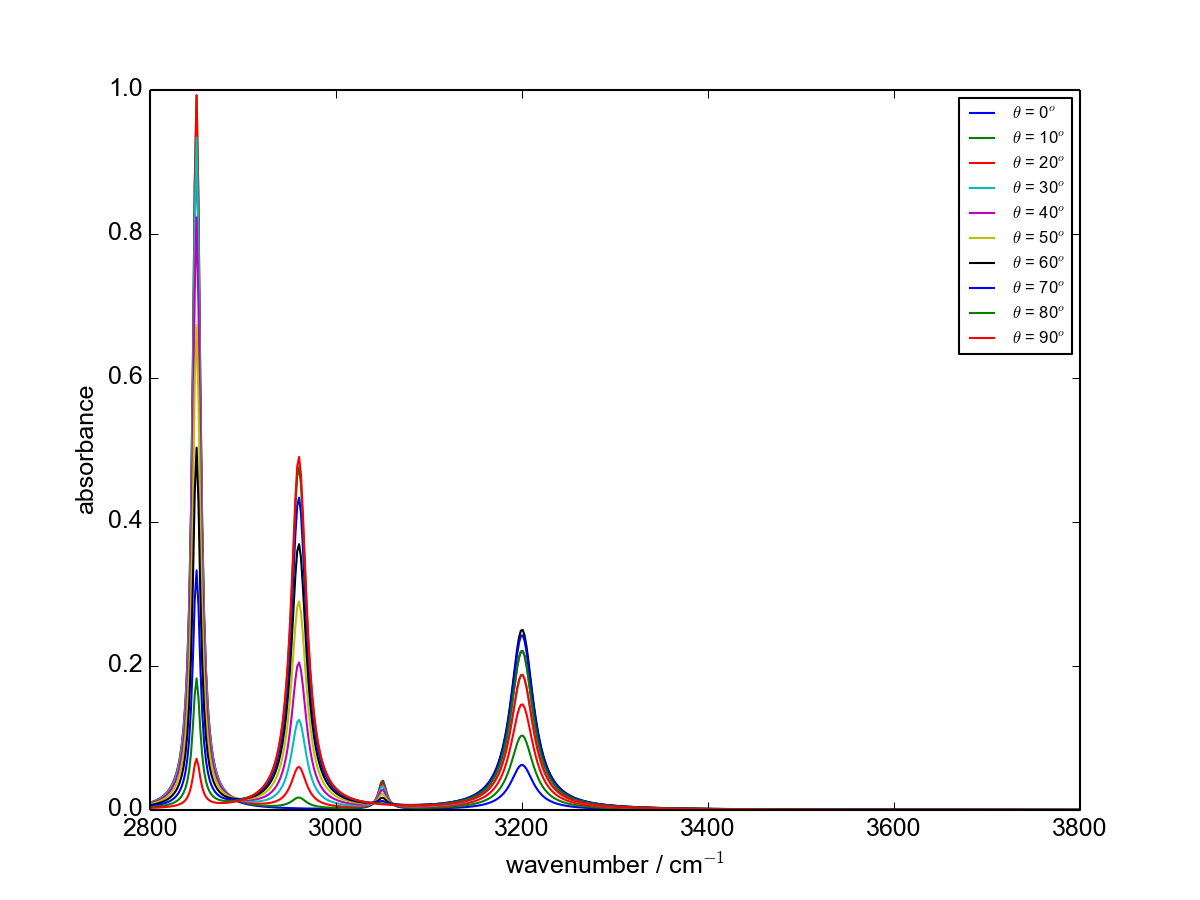
\includegraphics[scale=0.4]{Figures/Toy_Model_IR_Cosine_Projection.png} 
\caption{$cosine$- polarize IR spectra of toy model candidates} \label{fig:3.1}
\end{figure}

%A target spectrum is composed by combining $15$ percent of candidate with $\theta$ of $20^{\circ}$ and $85$ percent of candidate of $\theta$ of $70^{\circ}$: $0.15*f_{20}(x) + 0.85*f_{70}(x)$ in the following experiment. \\

\section{Linear Programming Model for Spectral Study}

Equation \ref{eq:3.2} is used to construct our LP model. The optimal solution returned by the LP solver is then compared with the target composition to see if they matches each other. This equation has also been used to study the composition of Ribonucleic acid (RNA) with ultraviolet (UV) spectra \cite{NYAS:NYAS900} and other UV spectroscopy studies  \cite{LPATUAS} back in the 60s. \\

\begin{eqnarray} \label{eq:3.2}
& \underset{p_{c}} {\text{minimize}} \displaystyle\sum^{\#~points}_{n=1} \left| Target- \displaystyle\sum^{\#~candidates}_{c=1}p_{c}f_{\theta}(x) \right| 
\end{eqnarray}
where $p_{c}$ are the unknown percentages for each candidate, which are the decision variables. $n$ is the number of points selected along the wavenumber, both for candidates and target spectra. $Target$ refers to the corresponding data points selected in target spectra. For each data point, the absolute residual between the target spectrum and the one composed by the decision variables is calculated. The objective function minimizes the sum of the absolute residuals over all the data points. \\

Because Equation \ref{eq:3.2} subjects to no restrictions, and the objection function is not in standard form. Getting rid of the absolute signs in the objective function is needed in order to use an LP approach. To eliminate the absolute sign is achieved by introducing one more variable $X$ and two more constraints for each data point as shown in Equation \ref{eq:3.3}. Then the previous model in Equation \ref{eq:3.2} is converted into the one in Equation \ref{eq:3.4} that can be solved by an LP solver. At last, one more constraint is introduced to restrict the sum of the percentages to be 1, as shown in Equation \ref{eq:3.4}. \\

For each point in the range of valid wavenumbers:
\begin{eqnarray} \label{eq:3.3}
& X = \left| Target-\displaystyle\sum^{\#~candidates}_{c=1}p_{c}f_{\theta}(x) \right| \nonumber \\
&  X \geq Target-\displaystyle\sum^{\#~candidates}_{c=1}p_{c}f_{\theta}(x)   \nonumber \\
& X \geq -Target+\displaystyle\sum^{\#~candidates}_{c=1}p_{c}f_{\theta}(x)  
\end{eqnarray} 

\begin{eqnarray} \label{eq:3.4}
& minimize \displaystyle\sum^{\#~points}_{n=1} X_p \nonumber \\
& X_1 - Target_1 + \displaystyle\sum^{\#~candidates}_{c=1}p_{c}f_{\theta}(x_1) \geq 0 \nonumber \\
& X_1 + Target_1 - \displaystyle\sum^{\#~candidates}_{c=1}p_{c}f_{\theta}(x_1) \geq 0 \nonumber \\
& ... \nonumber \\
& X_n - Target_n + \displaystyle\sum^{\#~candidates}_{c=1}p_{c}f_{\theta}(x_n) \geq 0 \nonumber \\
& X_n + Target_n - \displaystyle\sum^{\#~candidates}_{c=1}p_{c}f_{\theta}(x_n) \geq 0 \nonumber \\
& \displaystyle\sum^{\#~candidates}_{c=1}p_{c} = 1 
\end{eqnarray} 

Note that our LP model exactly describes our problem to be solved. Assuming that we can obtain sufficiently precise data, solving the LP will yield the target composition. Recall if the solution space is feasible and bounded, then there is a unique optimum solution. \\

\section{Linear Programming Model Implementation}

Next, we describe how to solve Equation \ref{eq:3.4} by implementing our LP model. Code is written to generate a file that contains all the candidates' spectral information needed for the experiments. For this step, the molecular properties files are used. For a specific candidate, given a molecular properties file and a $\theta$ value, the candidate's spectral information is obtained. For toy model, only the value of $\theta$ is needed, then Equation \ref{eq:3.1} is used to synthesize the spectral information. To further illustrate, a candidate class is written. This class defines candidate's $x$- and $z$-polarized IR spectra; $xx$-, $xy$-, $xz$-, and $zz$-polarized Raman spectra; $yyz$-, $yzy$-, $zzz$-polarized SFG spectra. Given a candidate's molecular properties and a $\theta$ value, a instance of this specific candidate is created. For the toy model, it only contains IR spectral information. Therefore, one candidate only contains $cosine$- and $sine$-polarized IR spectra. \\

In the second step, more code is written to generate a target composition of a list of needed candidates. Then the target composition is used to generate the target spectra. The probe range, which is the range of the wavenumber, is from 2800 to 3300 for toy model. The probe arrange is from $2000$ wavenumber to $3000$ wavenumber for real molecules. The target spectral information is generated in the same text file as candidate's spectral information. Depends on the experiment setting, code can be used to generate text files that contain different spectral information. \\

In the third step, the LP model is constructed by using the spectral information text file generated in the second step. This part of the code was written by Hung \cite{KuoKaiHung:Thesis:2015}. It reads all the candidates and target spectral information, and builds the LP model as shown in Equation \ref{eq:3.4}, then creates CPLEX LP input file. \\

In the fourth step, we use LP solver ``GNU linear progarmming tool kit" (GLPK) to read the CPLEX LP input file, then obtain the result. \\

\section{Experiments}

In Experiment 1 and 2, $4$ candidates are selected, the detailed setting is shown in Table \ref{tab:3.1}. In Experiment 1, there are $4$ candidates with $\theta$ of $0^{\circ}, 10^{\circ}, 20^{\circ}$, and $30^{\circ}$. In Experiment 2, the four candidates are with $\theta$ values of $0^{\circ}, 5^{\circ}, 10^{\circ}$, and $15^{\circ}$. Instead of having a $10$ degree variance in $\theta$, $5$ degree difference is applied on $\theta$ in Experiment 2. This means that when the candidates become more similar to each other than the ones in Experiment 1 as their spectra are more similar. In both experiments, 100 data points are selected evenly along the wavenumber from the spectra of $cosine$-polarized IR. The target composition of the candidates are the same for both experiments. In Experiment 1, the return composition is the same as the target one, however, the return composition for Experiment 2 does not match the target one. \\

\begin{table} 
\begin{center}
\begin{tabular}{| l | l | l | }
\hline
Experiment index & 1 & 2  \\
\hline
Number of Candidates & 4 & 4  \\
\hline
Candidates & [0, 10, 20, 30] & [0, 5, 10, 15] \\
\hline
Target Composition & [0.1, 0.5, 0.4, 0] & [0.1, 0.5, 0.4, 0]     \\
\hline
Number of Data Points & 100 from $cosine$-polarized IR &  100 from $cosine$-polarized IR     \\
\hline
Return Composition & [0.1, 0.5, 0.4, 0] & [0, 0.796962, 0.103038, 0.1] \\
\hline
\end{tabular} 
\end{center}
\caption{Experiment 1 and 2 setting using toy model}
\label{tab:3.1}
\end{table}	

In order to figure out why the return composition in Experiment 2 is different from the target one, the spectra generated by the return composition is plotted together with the target spectra as shown in Figure \ref{fig:3.2}. Note that the result spectra is almost identical to the target one. The residual between them is almost $0$. In order to see whether this observation is a general case, Experiment 3 is set up in Table \ref{tab:3.2}. Experiment 3 contains more candidates than Experiments 1 and 2. $10$ candidates are included with $\theta$ values ranging from $0^{\circ}$ to $90^{\circ}$.  \\

\begin{figure}[!ht] 
%\centering
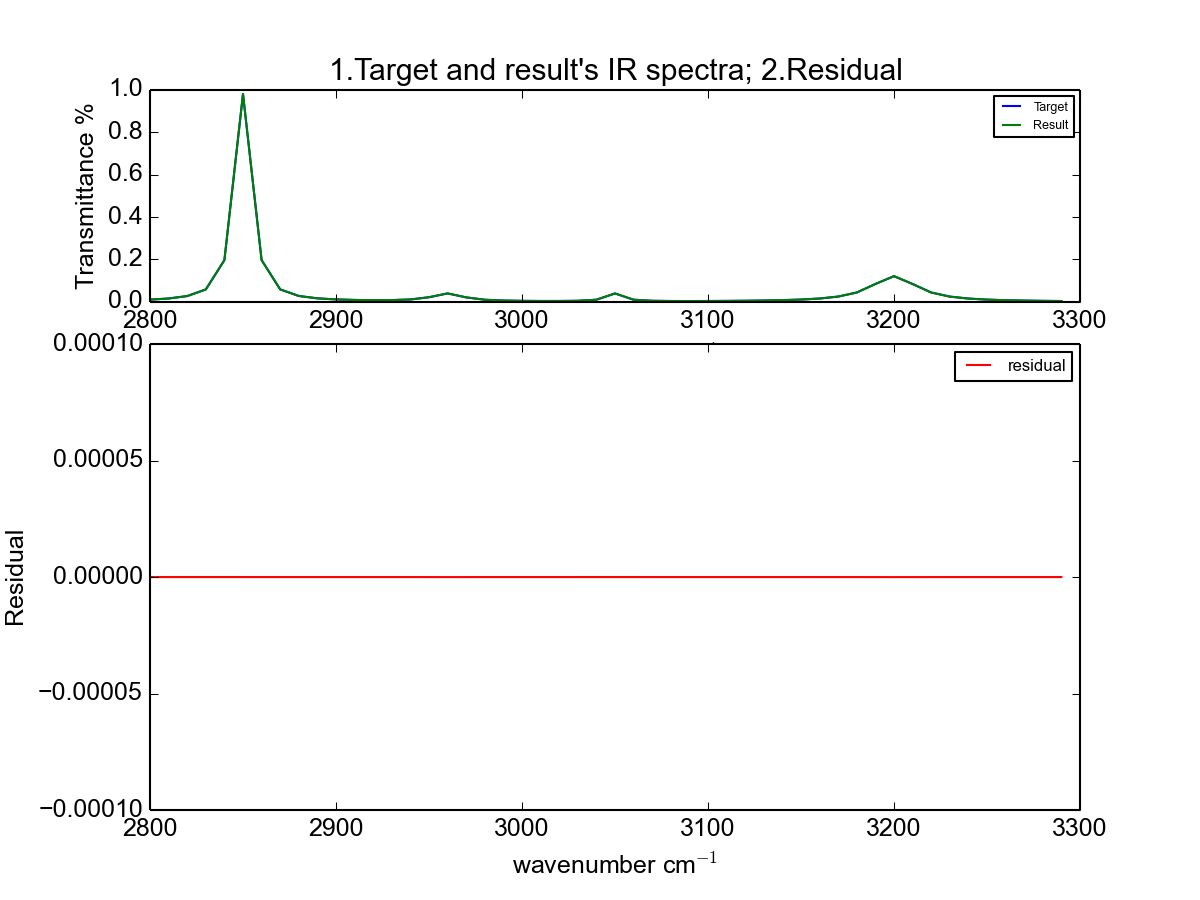
\includegraphics[scale=0.7]{Figures/toy_model_result_plotting_ir_cos_4candi_1.png}
\caption{Toy model Experiment 2 resulting $cosine$-polarized IR spectrum plotted with the target spectrum; and the residual plot between the spectra.}
\label{fig:3.2}
\end{figure}

\begin{table} 
%\begin{center}
\begin{tabular}{| l | p{7cm} | }
\hline
Experiment index & 3  \\
\hline
Number of Candidates & 10   \\
\hline
Candidates & [0, 10, 20, 30, 40, 50, 60, 70, 80, 90]  \\
\hline
Target Composition & [0.1, 0, 0.5, 0, 0.4, 0, 0, 0, 0, 0] \\
\hline
Number of Data Points & 100 from $cosine$-polarized IR \\
\hline
Return Composition & [0, 0, 0.730541, 0, 0.212061,0, 0, 0.0573978, 0, 0] \\
\hline
\end{tabular}
%\end{center}
\caption{Experiment 3 setting of toy model}
\label{tab:3.2}
\end{table}	

\begin{figure}[!ht] 
\centering
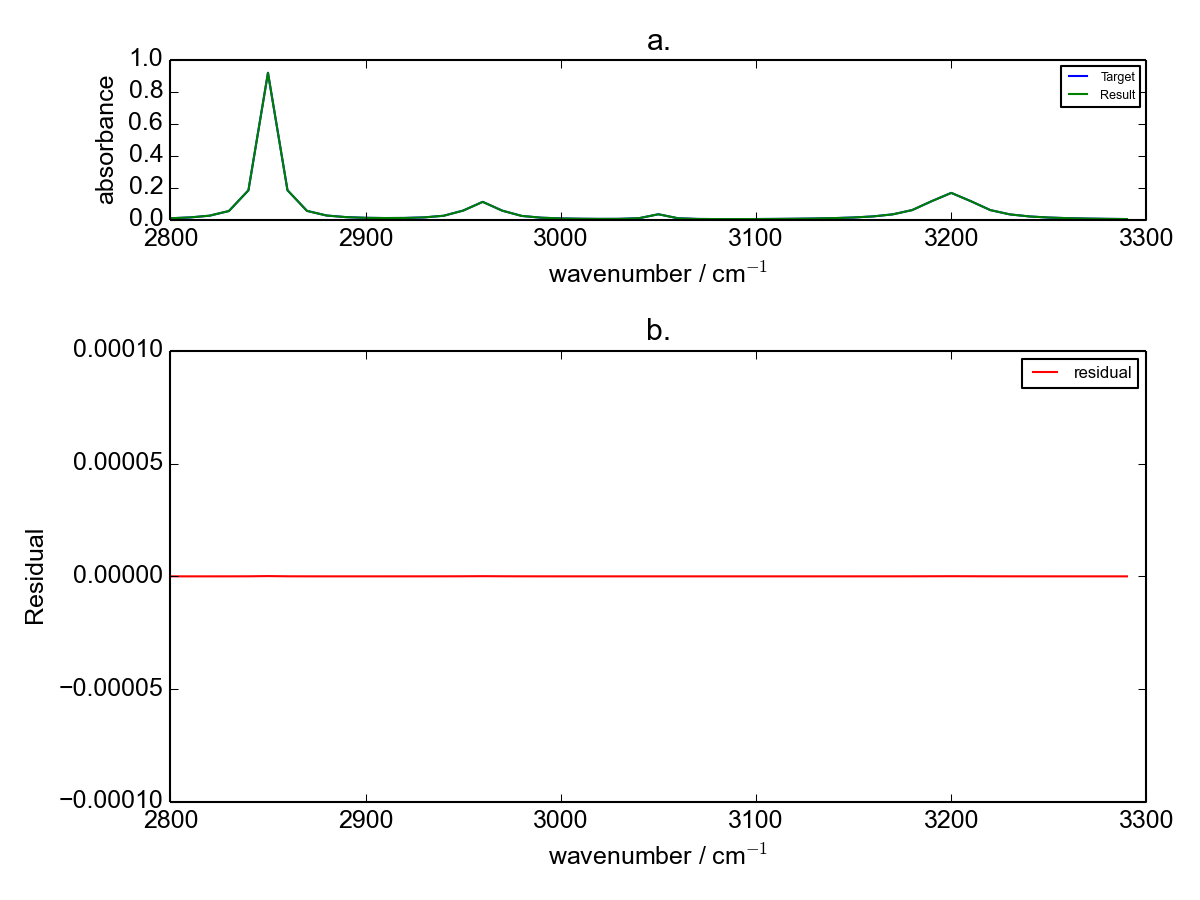
\includegraphics[scale=0.7]{Figures/toy_model_result_plotting_ir_cos_10candi_1.png} 
\caption{Toy model Experiment 3 resulting $cosine$-polarized IR spectrum plotted with target spectrum; and the residual plot between the two spectra}
\label{fig:3.3}
\end{figure}

Table \ref{tab:3.2} indicates the return composition of Experiment 3 is different from the target one. Figure \ref{fig:3.3} shows that the spectrum produced by the return composition is almost identical to the one generated by the target composition in Experiment 3. The residual is negligible as well. This observation is the same as Experiment 2. \\

Among Experiment 1, 2 and 3, only the return composition of Experiment 1 matches its target one. However, in Experiment 2, the difference in $\theta$ value among the candidates is smaller than Experiment 1. In Experiment 3, the number of the candidates is larger than Experiment 1. Both effects increase the complexity of the experiments. In both Experiment 2 and 3, the spectrum constructed by the return composition matches to the one built by the target composition. \\

The above observation demonstrates that there are multiple compositions can achieve in constructing the spectrum that are close to the target one. The numerical limitation helps the LP solver to converge to a unique optimum solution. The reason for Experiment 1 to return a composition that matches to the target one, is that the spectral information used to construct the LP model is competent. The constraints constructed in the LP model of Experiment 1 eventually converge to the target composition. \\ 

%the corresponding LP model, built with the presenting spectral information, may lack of competent information to guarantee the return composition actually  is the target one. Because of the high complexity in the setting of the candidates pool, the solution for the LP model may not be unique. However, in real LP problem solving, the numerical limitation helps LP solver to converge to an unique solution. This unique solution is the optimum one for the LP model with the information currently available. Further demonstration will also be expanded in Chapter \ref{ch:4} when real molecules are introduced. \\ %the complexity of Experiment 2 and 3 is higher than Experiment 1.\\

In order to add necessary information to construct the constraints in our LP model, IR's second polarization is introduced to the toy model: the $sine$ polarization. Figure \ref{fig:3.4} describes how the $sine$-polarized spectra presented for $10$ candidates. Experiment 4 and 5 include both polarizations' spectral information in the LP model. In Table \ref{tab:3.3}, Experiment 4's setting is based on Experiment 2, with $sine$-polarized IR spectral information added. $100$ data points are selected from this additional spectrum, then converted to additional decision variables and constraints in the LP model. Same with Experiment 5, it is based on Experiment 3, with sine-polarization IR spectral information added. For both Experiment 4 and 5, the return composition now matches to the target one. This further proves that as long as we have sufficing information to build the constraints, the LP solver will return a composition matches to the target one. \\ 

\begin{figure}[!ht]
\centering
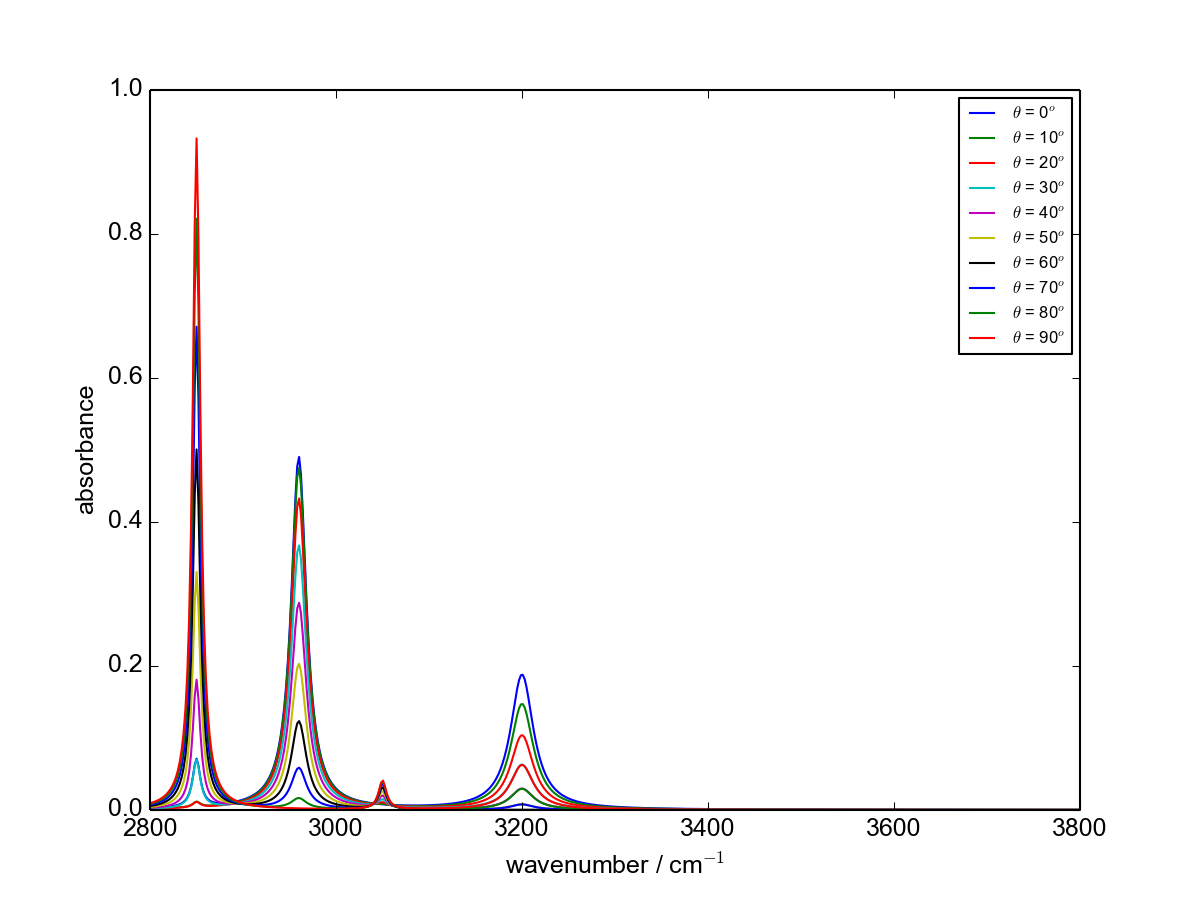
\includegraphics[scale=0.7]{Figures/Toy_Model_IR_Sine_Projection.png} 
\caption{$sine$-polaried IR spectra of toy model candidates with $\theta$ value expanded from $0^{\circ}$ to $90^{\circ}$}  \label{fig:3.4}
\end{figure}

\begin{table} \small 
\begin{center}
\begin{tabular}{| l | p{5cm} | l |}
\hline
Experiment index & 4 & 5\\
\hline
Number of Candidates & 4 & 10 \\
\hline
Candidates & [0, 5, 10, 15] & [0, 10, 20, 30, 40, 50, 60, 70, 80, 90] \\
\hline
Target Composition & [0.1, 0.5, 0.4, 0] & [0.1, 0, 0.5, 0, 0.4, 0, 0, 0, 0, 0]\\
\hline
Number of Data Points & 100 from $cosine$-polarized IR + 100 from $sine$-polarized IR & 100 from $cosine$-polarized IR + 100 from $sine$-polarized IR\\
\hline
Return Composition & [0.1, 0.5, 0.4, 0] & [0.1, 0, 0.5, 0, 0.4, 0, 0, 0, 0, 0] \\
\hline
\end{tabular} 
\caption{Experiment 4 and 5 setting of toy model}\label{tab:3.3}
\end{center}
\end{table}		

\section{Constraint Study Based on Experiment 4}

From Experiment 1 to 5, we know having sufficient information in our LP model is the key to obtain the target composition. Having sufficient information means having enough constraints to help LP model converge to a desired result. Moreover, the information is coming from the valuable data points selected along the spectra. This leads us to do a further study on the constraints in order to see how many data points are enough to get the desired composition.\\ 

Based on Experiment 4, experiments about formulating the LP model with different data information are conducted in Table \ref{tab:3.4}. The number of data points indicates how many data points are selected. Points Selection shows how data points are selected. [2800, 3300, 50] means along wavenumber from 2500 to 3300, every 25 wavenumber. For example, Experiment 6 contains 10 data points from $cosine$- polarized IR spectrum. Every 50 wavenumber, one data point is selected. Similarly, for Experiment 7, 8, 9, 10, 11, every 25, 20, 15, 10 and 5 wavenumber, one data point is select. From Experiment 12 to 16, data points are selected from both cosine-polarized and sine-polarized IR spectrum. \\

(TODO: rethink: What can we exactly get from the following two tables? Should we include this study?)

\begin{table} \small
\begin{center}
\begin{tabular}{| l | l | p{3cm} | l |} \hline
	Experiment Index & Number of Data Points & Points Selection & Result \\ \hline
	6 & 10 & [2800, 3300, 50] & [0, 0.796962, 0.103038, 0.1] \\ \hline
	7 & 20 & [2800, 3300, 25] & [0, 0.796962, 0.103038, 0.1] \\ \hline
	8 & 25 & [2800, 3300, 20] & [0, 0.796962, 0.103038, 0.1] \\ \hline
	9 & 32 & [2800, 3300, 15] & [0, 0.796962, 0.103038, 0.1] \\ \hline
	10 & 50 & [2800, 3300, 10] & [0, 0.796962, 0.103038, 0.1] \\ \hline
	11 & 100 & [2800, 3300, 5] & [0, 0.796962, 0.103038, 0.1] \\ \hline
	12 & $100 + 1$ & [2800, 3300, 5], [2800, 3300, 500] & [0, 0.796962, 0.103038, 0.1] \\ \hline
	13 & $100 + 5$ & [2800, 3300, 20], [2800, 3300, 100] & [0, 0.796962, 0.103038, 0.1] \\ \hline
	14 & $100 + 10$ & [2800, 3300, 20], [2800, 3300, 50] & [0, 0.796962, 0.103038, 0.1] \\ \hline
	15 & $100 + 50$ & [2800, 3300, 20], [2800, 3300, 10] & [0.1, 0.5, 0.4, 0] \\ \hline
	16 & $100 + 100$ & [2800, 3300, 20], [2800, 3300, 5] & [0.1, 0.5, 0.4, 0] \\ 
	\hline
\end{tabular} 
\end{center}
\caption{Constraint Study Based on Experiment 4} \label{tab:3.4}
\end{table}

One interesting result from Table \ref{tab:3.4} is that: from Experiment 1 to 9, the result composition is the same. To the contrary, from Experiment 10, the return composition gets changed to the target one. Furthermore, if we plot the return composition of [0, 0.796962, 0.103038, 0.1] and the target one [0.1, 0.5, 0.4, 0] in  Picture \ref{fig:3.5}. In this picture, we can see that the spectra generated by these two composition are identical.

\begin{figure}[!ht] 
\centering
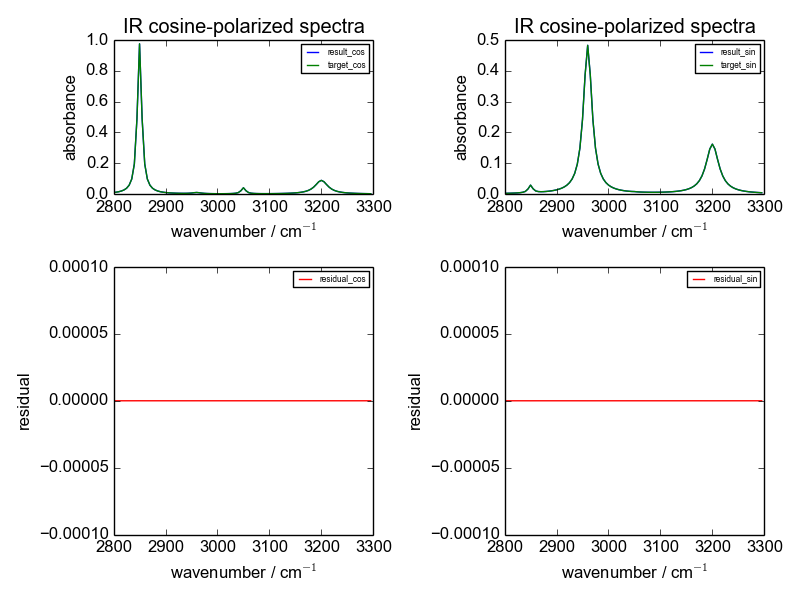
\includegraphics[scale=0.3]{Figures/toy_model_result_plotting_ir_sin_4candi_constraint_study_experiment4.png} 
\caption{Toy Model Constraint Study 1}\label{fig:3.5}
\end{figure}


\section{Constraint Study Based on Experiment 5}

When the same constraint study is applied to the data based on Experiment 5 in Table \ref{tab:3.6}, the observation is the same as the experiments in Table \ref{tab:3.4}. This further proves that: We can obtain different solutions by have different constraints. When the  result composition [0, 0, 0.730541, 0, 0.212061,0, 0, 0.0573978, 0, 0] and target one [0.1, 0, 0.5, 0, 0.4, 0, 0, 0, 0, 0] are plotted together, they are almost identical as well, as shown in Figure \ref{fig:3.6}.

\begin{table} \tiny 
\begin{center}
\begin{tabular}{| l | l | p{3cm}  | p{6cm} |}
\hline
Experiment Index & Points & Point Selection & Result \\ \hline
17 & 10 & [2800, 3300, 50] & [0.156758, 0, 0, 0.825977, 0, 0, 0, 0, 0, 0.017265] \\ \hline
18 & 25 & [2800, 3300, 20] & [0, 0, 0.730541, 0, 0.212061, 0, 0, 0.0573978, 0, 0, 0] \\ \hline
19 & 50 & [2800, 3300, 10] & [0, 0, 0.730541, 0, 0.212061, 0, 0, 0.0573978, 0, 0, 0] \\ \hline
20 & 100 & [2800, 3300, 5] & [0, 0, 0.730541, 0, 0.212061, 0, 0, 0.0573978, 0, 0, 0] \\ \hline
21 & 500 & [2800, 3300, 5] & [0, 0, 0.730541, 0, 0.212061, 0, 0, 0.0573978, 0, 0, 0] \\ \hline	
22 & $100 + 1$ & [2800, 3300, 5], [2800, 3300, 500] & [0, 0, 0.730541, 0, 0.212061, 0, 0, 0.0573978, 0, 0, 0] \\ \hline
23 & $100 + 10$ & [2800, 3300, 5], [2800, 3300, 50] & [0.361587, 0, 0.312061, 0.326352, 0, 0, 0, 0, 0] \\ \hline
24 & $100 + 20$ & [2800, 3300, 5], [2800, 3300, 25] & [0.174023, 0, 0, 0.791447, 0, 0, 0.0345301, 0, 0, 0] \\ \hline
25 & $100 + 25$ & [2800, 3300, 20], [2800, 3300, 20] & [0.174023, 0, 0, 0.791447, 0, 0, 0.0345301, 0, 0, 0] \\ \hline
26 & $100 + 50$ & [2800, 3300, 5], [2800, 3300, 10] & [0, 0, 0.753209, 0, 0.146791, 0, 0.1, 0, 0, 0] \\ \hline
27 & $100 + 84$ & [2800, 3300, 5], [2800, 3300, 6] & [0.174023, 0, 0, 0.791447, 0, 0, 0.0345301, 0, 0, 0] \\ \hline
28 & $100 + 100$ & [2800, 3300, 5], [2800, 3300, 5] & [0.1, 0, 0.5, 0, 0.4, 0, 0, 0, 0, 0] \\ 
\hline
\end{tabular} \\
\caption{Constraint Study Based on Experiment 5}\label{tab:3.6}
\end{center}
\end{table}

\begin{figure}[!ht] 
\centering
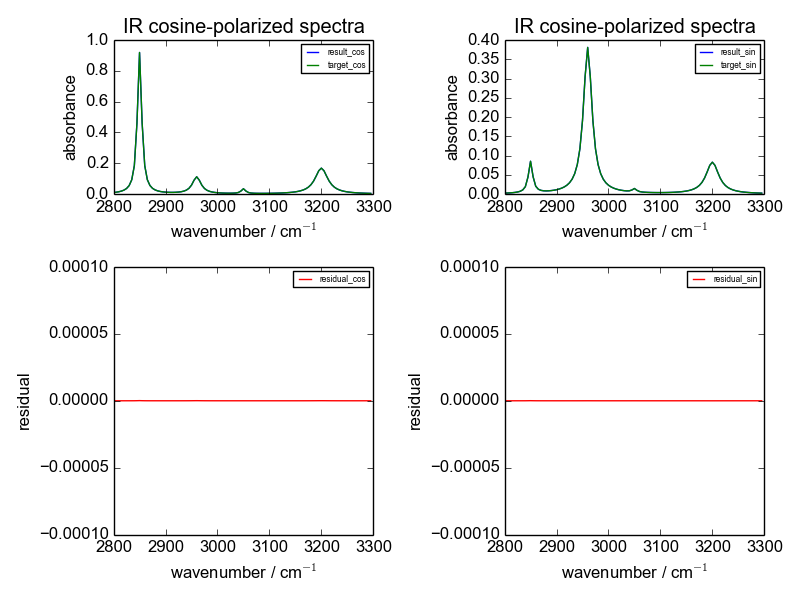
\includegraphics[scale=0.3]{Figures/toy_model_result_plotting_ir_sin_10candi_constraint_study_experiment5.png} 
\caption{Toy Model Constraint Study 2}\label{fig:3.6}
\end{figure}

\section{Discussion and Conclusion}
With all the experiments conducted with the toy model, we have learnt that the reason, that our LP model does not return a composition that matches the target one, is that the model does not have sufficient information to build the constraints. However, with the limited information, the optimal solution returned by our LP model does build the perfect target spectrum. This means that the solution for the composition that achieves minimum residual of the objective function is not unique. However, in real experiment, because numerical restriction, an unique optimal solution is obtained from the LP model. \\

Above analysis simulates the following question: how can we know there is enough information to achieve the target composition? In the next step, we will experiment with real molecules. The goal is to investigate with all the spectral information that we can obtain for real molecules, can our LP model return the target composition for the target spectrum? If yes, can we apply the LP model systematically? Furthermore, to maximally explore the capacity of our LP model, and study its limitation. Finally, come up with some general instructions for applying our LP model. These are the main focus for the following chapters.\\

		

		 



